\documentclass[a4paper, 10pt, american]{article}
\usepackage[utf8]{inputenc}
\usepackage{csquotes}
\usepackage{bookmark}
\usepackage{hyperref}
\usepackage[american]{babel}
\usepackage[margin=1in]{geometry}
\usepackage{setspace}
\usepackage{multirow}
\usepackage{graphicx}
\usepackage{wrapfig}
\usepackage[inline]{enumitem}
\usepackage{lipsum}
\usepackage{listings}
\usepackage[dvipsnames]{xcolor}
\graphicspath{{./images/}}
\newcommand{\etal}{et~al. }

\hyphenation{smart-phones smart-phone}

\lstdefinelanguage{Kotlin}{
  comment=[l]{//},
  commentstyle={\color{gray}\ttfamily},
  emph={filter, first, firstOrNull, forEach, lazy, map, mapNotNull, println},
  emphstyle={\color{OrangeRed}},
  identifierstyle=\color{black},
  keywords={!in, !is, abstract, actual, annotation, as, as?, break, by, catch, class, companion, const, constructor, continue, crossinline, data, delegate, do, dynamic, else, enum, expect, external, false, field, file, final, finally, for, fun, get, if, import, in, infix, init, inline, inner, interface, internal, is, lateinit, noinline, null, object, open, operator, out, override, package, param, private, property, protected, public, receiveris, reified, return, return@, sealed, set, setparam, super, suspend, tailrec, this, throw, true, try, typealias, typeof, val, var, vararg, when, where, while},
  keywordstyle={\color{NavyBlue}\bfseries},
  morecomment=[s]{/*}{*/},
  morestring=[b]",
  morestring=[s]{"""*}{*"""},
  ndkeywords={@Deprecated, @JvmField, @JvmName, @JvmOverloads, @JvmStatic, @JvmSynthetic, Array, Byte, Double, Float, Int, Integer, Iterable, Long, Runnable, Short, String},
  ndkeywordstyle={\color{BurntOrange}\bfseries},
  sensitive=true,
  stringstyle={\color{ForestGreen}\ttfamily},
}

\title{Thesis Proposal}
\author{Joseph Petitti}
\date{November 17, 2020}

\begin{document}

\begin{titlepage}
\begin{center}
\doublespacing


{\Large \textsc{Appjudicator}: \\
Enhancing Android Network Analysis through UI Monitoring}

\vfill

by \par

Joseph Petitti

\vfill

A Thesis \\
Submitted to the Faculty \\
of the \\
WORCESTER POLYTECHNIC INSTITUTE \\
In partial fulfillment of the requirements for the \\
Degree of Master of Science \\
in \\
Computer Science \par

\vfill

by

\vspace{0.55cm}

\underline{\hspace{3in}} \\

May 2021

\end{center}

\vfill

\begin{flushleft}
APPROVED: \par
\vspace{\baselineskip}

\underline{\hspace{3in}} \\
Professor Craig A. Shue, Major Thesis Advisor \par
\vspace{\baselineskip}

%\underline{\hspace{3in}} \\
%Professor [TBD] Thesis Reader \par
%\vspace{\baselineskip}

\underline{\hspace{3in}} \\
Professor Craig E. Wills, Head of Department \par
\end{flushleft}
\end{titlepage}

\pagenumbering{roman}

\begin{abstract}
	Smartphones are becoming increasingly important in all aspects of life,
	including corporate environments, where ``bring your own device'' (BYOD)
	policies are gaining widespread acceptance. Malware already exists to take
	advantage of Android phones in BYOD settings, aiming to take control of
	devices with access to privileged information by disguising itself as a
	benign app. Malware could be easier to detect if network administrators had
	more insight into employee-owned smartphones. We propose a system, called
	\textsc{Appjudicator}, to address this issue. It implements an accessibility
	service to monitor user interactions with the user interface (UI) of other
	apps, so this context can be used in malware detection. For example, if an
	app sends a new network request without any user interaction, this flow
	could be the result of malware and should be investigated. Our app is a
	host-based software defined networking (SDN) agent that works in conjunction
	with an SDN controller to monitor and control the phone's networking
	abilities based on the organization's SDN rules and our UI context. We build
	a proof of concept application and find that it can successfully combine
	network and UI data with only 10 milliseconds of total added latency in 95\%
	of flows.
\end{abstract}

\clearpage

\section*{Acknowledgments}
\label{sec:acknowledgments}

I would like to express my gratitude to my advisor, Professor Craig Shue, for
guiding me through my graduate education with helpful advice and insightful
feedback. Without his patience and wisdom this thesis could not have happened. I
would also like to thank Yu Liu for his technical help and support throughout
the project, along with Matt Puentes and Cole Granof for their advice and moral
support. I also wish to thank Beckey Schowalter for her help with writing and
grammar. Additionally, I want to express my appreciation to my thesis reader,
Professor Robert Walls, for his helpful feedback on this project. His questions
and criticism, along with those from every member of the WPI Cake Lab, are what
turned this paper from a very rough summary to a polished final product.

\clearpage

\tableofcontents

\clearpage
\pagenumbering{arabic}


\section{Introduction}
\label{sec:introduction}

% Need

Current corporate network administration tools have little insight into the
connections made by employee-owned smartphones, especially in ``Bring Your Own
Device'' (BYOD) scenarios that are becoming increasingly common. It is difficult
for large organizations to maintain security across their networks with such
little knowledge about, and control over, these mobile devices. The fact that
these devices enter and exit the corporate network and connect to other
networks, such their cellular data provider's, on a daily basis complicates this
issue. Smartphones have a wide range of powerful networking and computational
abilities, and are typically privately owned by employees, which raises further
concerns when integrating them into secure network environments.

For example, smartphones have been targeted by malware specifically designed to
infiltrate corporate networks~\cite{kan2016}, such as ``Dresscode'', which
disguises itself as a legitimate app in order to steal data and add infected
devices to a botnet~\cite{palmer2016}. The ``xHelper'' malware can automatically
download and install arbitrary software specified by an attacker, and persists
even after a factory reset~\cite{vijayan2020}. A black market
malware-as-a-service model called Black Rose Lucy even offers control of
infected Android devices to paying customers, potentially giving any malicious
actor an entry point to a secure network~\cite{wong2018}.

If mobile devices are to have access to sensitive corporate network
infrastructure, either from home or from work, administrators need new tools to
monitor and control their network connections. These tools need to be powerful
enough to detect when network connections are made by Trojan horse malware that
is disguised as a benign app, while being still being easy to deploy and manage.
For example, some existing solutions require recompiling Android's kernel or
gaining root access to their device, which is impractical for most users and
exposes them to additional security risks~\cite{google2020}.

% Approach

To solve these issues on Android devices, we propose a new app called
\textsc{Appjudicator} which leverages user interface (UI) interaction and
software-defined networking (SDN) principles to determine whether network flows
are legitimately user-initiated. The app has two components: an accessibility
service that monitors UI interaction and a VPN service that intercepts network
flows and acts as an OpenFlow agent. We use these two sources of information to
correlate network flows with user interaction in a way that is difficult for
malware to evade, since it cannot physically interact with hardware input
devices.

The UI monitoring component will use Android's accessibility API to
asynchronously record physical hardware inputs, such as tapping or swiping the
touch screen. This gives administrators the ability to accurately distinguish
between human-driven and automated network requests.  Meanwhile, the VPN service
acts as an OpenFlow agent and rule cache, giving administrators fine-grained
control over which connections the device is allowed to make. Flows are
augmented with context from the specific device and application, and can be
elevated to the organization's SDN controller if necessary.

% Benefit over cost

Our application provides organizations with a new set of powerful, easy to use
tools for monitoring BYOD Android smartphones in a simple app package that is
easy for users to install. It does not require rooting, recompiling the kernel,
or any other cumbersome processes. It can distinguish between user-generated and
automated network requests with a high degree of confidence using techniques
that are difficult for malware to evade. This makes users safer by detecting
stealthy malware on their devices, and improves the organizations network
security.

The costs of our system include the resource overhead of running the app (CPU
cycles, battery power, etc.) and the cost of installing, running, and
maintaining the controller server. We expect these costs to be a relatively
small addition to existing resources. The app's UI monitoring and VPN service
also add some latency to network requests performed on the phone. In our
experiments \textsc{Appjudicator} added less than 100 milliseconds of total
latency to new TCP connections in 97\% of trials. UDP connections and subsequent
TCP requests to established connections have even less added latency.

% TODO can we justify this latency?

% Competition

Using UI data to distinguish user-initiated behavior and the use of a smartphone
as an SDN agent have been studied by others before, but \textsc{Appjudicator}
combines these aspects in new and important ways. Android host-based SDN agets
have been investigated by Hanguard~\cite{demetriou2017}, and using UI
interaction as context for identifying malicious app behavior was examined in
AppIntent~\cite{yang2013}, but our system combines these approaches to form a
novel solution for a distinct use case. One key difference is that AppIntent
uses machine learning to conduct static analysis of apps, while
\textsc{Appjudicator} enables live monitoring and response to malicious network
flows in real time.

Kwon~\etal have proposed a system that uses UI data to distinguish
user-generated network flows, and the combination of UI monitoring and SDN has
been implemented on Microsoft Windows by Harbinger~\cite{chuluundorj2019}.  We
solve new challenges by implementing this strategy on the Android platform. For
example, we are constrained by Android's rigid permissions system, we do not
have root access to the device, and we cannot modify the kernel. These
restrictions require novel techniques and systems.

Our work focuses on exploring the following research question: 
\begin{quote}
	\textit{Can UI interaction and network activity be used to successfully
		predict and associate network flows with user actions on Android devices
		with acceptable overhead?}
\end{quote}

To investigate we perform a study with several popular Google Play apps to
determine whether \textsc{Appjudicator} can successfully detect and block
suspicious non-user-initiated network requests. % TODO insert results
We also measure the total added latency of the VPN and SDN agent, finding that
our system adds less than 10 milliseconds of total end-to-end latency to 95\% of
intercepted packets. On a standard 60 Hz screen this latency is imperceptible to
users.

% TODO add more results

\newpage

\section{Background and Related Work}
\label{sec:related-work}

Related work has been conducted in both of the main focus areas of this project:
the use of UI interaction data for security and implementing SDN on the Android
platform. We now review such work.

\subsection{UI Interaction and Security}
\label{sec:ui-interaction-and-security}

Previous work has investigated how user interactions with the UI can be used to
identify human-initiated behavior on various platforms. Harbinger examines user
interface activity on Windows to provide context for network requests to
previously unknown hosts in a default-deny environment~\cite{chuluundorj2019}.
This approach ``hooks into'' mouse and keyboard inputs using Microsoft's UI
Automation library~\cite{microsoft2018}, intercepting the input before it is
received by the intended application. Although Harbinger's operations are
performed synchronously they still only added six milliseconds or less of
latency to 96\% of flows. In contrast, the relevant library on Android is
asynchronous and event-driven~\cite{googledevelopers2020}.

Kwon \etal also used UI interaction data to distinguish human-generated from
automated network requests on Windows~\cite{kwon2011}. They propose a host-based
system for combating botnets by leveraging UI interaction data. But their
approach of labelling any flow initiated within one second of an interaction
with the flow's process as ``user generated'' ignores much of the context that
can be gained from UI data and makes deliberate evasion easy.

Most previous work on Android has used the platform's
\textit{AccessibilityService}, a library that includes the ability to respond to
UI changes among other accessibility features. AppIntent~\cite{yang2013} uses
this service to determine if an app is leaking private information by building a
graph of UI interactions that could lead to information leakage. However,
AppIntent is only designed to determine whether an app \textit{could} leak
private information through static analysis, and does not work in real time on a
flow-to-flow basis.

% SDN in general section
\subsection{Software-defined Networking}
\label{sec:software-defined-networking}

Software-defined networking (SDN) has been studied as a tool for giving network
administrators more information about, and control over, intra-network traffic.
In essence, SDN centralizes network intelligence by separating the forwarding of
packets (the data plane) from their routing (the control plane). In this
paradigm network switches merely forward packets, while all control and logic is
centralized with an SDN controller server~\cite{kim2013}.

SDN gives administrators more fine-grained control over packet routing rules,
which enables more sophisticated policy enforcement. It also provides insight
into potential issues and congestion in the network from one centralized control
point, rather than spread across many switches and routers. The main drawback of
this approach is the high overhead that causes it to scale
poorly~\cite{benzekki2016}.

Some authors have investigated using end nodes, instead of routers and switches,
as SDN rule caches to alleviate this problem~\cite{taylor2017, chuluundorj2019}.
In this approach, each host caches rules from the SDN controller and makes
routing decisions about its own network flows.

Others have investigated the potential for improving SDN's capabilities by
adding context~\cite{yang2015}, an approach which \textsc{Appjudicator} also
attempts. SDN rules could be more powerful and granular with more metadata, for
example a network flow's initiating application.

\subsection{The Android Phone as an SDN Agent}
\label{sec:the-android-phone-as-an-sdn-agent}

Many previous applications have used an Android smartphone as a SDN agent and
rule cache. Hong~\etal explores the tools available to organizations for
managing BYOD Android devices and proposes a system for applying SDN policies to
these phones~\cite{hong2016}. They were able to apply app-specific rules that
were aware of device context such as GPS location with minimal overhead.

While Hong~\etal \cite{hong2016} was aimed at corporate users, HanGuard
investigated using SDN principles to protect Internet of things (IoT) devices in
home networks~\cite{demetriou2017}. Their application provided tools for users
to easily define SDN rules for IoT apps, IoT devices, and users.

While each of these areas has been extensively researched alone, only
Chuluundorj~\cite{chuluundorj2019} and Kwon~\etal \cite{kwon2011} have
investigated how UI and network data can be combined for security purposes.
However, both of these applications were developed for the Windows
platform---bringing the idea to Android involves a new set of constraints and
challenges. For example, our proposed solution can be installed as a normal app,
and does not require recompiling the kernel or rooting the phone. This means
that we cannot modify the operating system kernel as the Windows solutions do,
and must abide by Android's strict permissions system.

\newpage

\section{Approach and Implementation}
\label{sec:implementation}

\textsc{Appjudicator} works by analyzing network flows with the added context of
UI interaction data. It uses this information as part of a host-based
software-defined networking (SDN) agent to make decisions about whether to allow
or block individual flows. The app is composed of three primary components:
\begin{enumerate*}[label=(\arabic*)]
	\item a VPN service that captures and analyzes network flows from the
		device,
	\item an accessibility service that monitors user interactions with the
		UI, and
	\item an SDN agent that implements a subset of the OpenFlow 1.0
		specification~\cite{openflowspec}.
\end{enumerate*}

\begin{wrapfigure}{R}{0.4\textwidth}
	\centering
	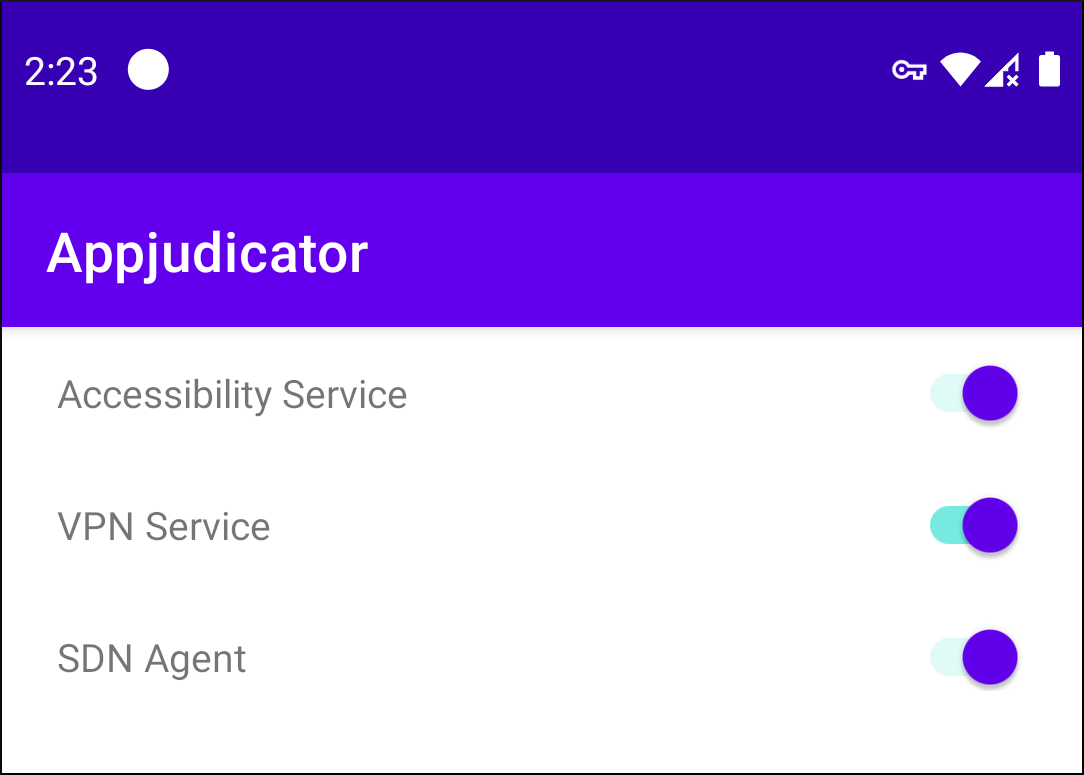
\includegraphics[width=0.4\textwidth]{ui-screenshot-border.png}
	\caption{A screenshot of \textsc{Appjudicator}'s user interface (vertical
		whitespace truncated for brevity).}
	\label{fig:ui-screenshot}
\end{wrapfigure}


The app is implemented using Kotlin, an object-oriented programming language
that is interoperable with Java and compiles to Java Virtual Machine bytecode.
This is Google's preferred language for Android development, and makes some
tasks like null-checking and concurrency easier than they would be in
Java~\cite{lardinois2019}. As a proof of concept, the app's user interface is
minimal, simply providing a list of which services are running and a method to
toggle them (see Figure~\ref{fig:ui-screenshot}).

The VPN service implements Android's \texttt{VpnService}
API~\cite{googledevelopers2020vpn}, but connects to a packet-capturing class
running on the same phone rather than a remote server. The UI-monitoring
component implements Android's \texttt{AccessibilityService}
API~\cite{googledevelopers2020}, and the SDN agent implements a subset of the
OpenFlow 1.0 switch standard~\cite{mckeown2008}. Each of these components work
together to correlate network flows with a UI interaction (or lack thereof) that
initiated them, and elevate suspicious flows to the SDN controller. We now
describe each of these components and explain how they work together.

\subsection{VPN Service}
\label{sec:implementation-vpn-service}

The networking component of \textsc{Appjudicator} utilizes Android's built-in
API for redirecting network traffic, the
\texttt{VpnService}~\cite{googledevelopers2020vpn}. However, rather than connect
to a remote VPN server, we connect to a simple server running locally on the
device. We register a new VPN connection using this API and prompt the user to
connect to it. This routes all the device's traffic through our service, which
captures and logs packets before forwarding them along to their destination.

Once activated, the VPN service runs in the background and receives packets from
the operating system through a \texttt{ParcelFileDescriptor} instance that can
be used to read and write packets from the network interface's
buffer~\cite{vpnguide}.  Normally, a VPN service would forward packets through a
tunnel to a remote VPN server, but \textsc{Appjudicator}'s VPN server runs
locally on the device.  Packets are instead passed to processes running on other
threads that log the packets and forward them along to their destination using
Java sockets.

It is normally the app's responsibility to encrypt data being transferred to the
VPN gateway~\cite{vpnguide}, but this is unnecessary in \textsc{Appjudicator}
because both client and server are running on the same device. We benefit from
reduced computational resource consumption and energy use from from not having
to encrypt and decrypt packets.

\subsubsection{Deconstructing Flows}
\label{sec:deconstructing-flows}

Captured packets are parsed, logged, and reconstructed by the VPN service using
Pcap4J, a third-party Java IP packet library~\cite{kaito2016}. Source and
destination IP addresses are collected from the packet's IP header, along with
source and destination ports from the TCP or UDP header. \textsc{Appjudicator}
currently only supports IPv4, so any intercepted IPv6 packets are simply
dropped. Likewise, packets with unknown transport-layer protocols
(\textit{i.e.}, neither TCP nor UDP) are dropped. The network context provided
by the VPN service includes IP source and destination addresses, protocol,
source and destination ports, payload size, initiating application, and full
packet payload, all of which can be used to enforce fine-grained SDN rules.

\textsc{Appjudicator} associates an app with the flows it created.  On Android
API versions Q and later we can use the \texttt{ConnectivityManager} to query
the operating system for which user ID owns a particular flow. Because each app
has a different user ID in Android, we can then use the \texttt{packageManager}
to look up the package name for that UID as long as we requested the
\texttt{QUERY\_ALL\_PACKAGES} permission. See Listing~\ref{lst:connToPackage}
for an example of how to do this in Kotlin.

\begin{figure}[h]
\begin{lstlisting}[caption={Source code to obtain the package that created a
		given network flow.},
	label={lst:connToPackage}, language=Kotlin]
@RequiresApi(Build.VERSION_CODES.Q)
fun connToPackage(
    protocol: Int, // either TCP (6) or UDP (17)
    localAddress: InetSocketAddress,
    remoteAddress: InetSocketAddress,
    context: Context
): String {
	val cm = context.getSystemService(Context.CONNECTIVITY_SERVICE)
			as ConnectivityManager
	val uid = cm.getConnectionOwnerUid(
		protocol,
		localAddress,
		remoteAddress
	)
	if (uid == android.os.Process.INVALID_UID) return "unknown"
	return context.packageManager.getNameForUid(uid) ?: "unknown"
}
\end{lstlisting}
\end{figure}

Packets are organized by flow, essentially a communication channel between one
application and another. A flow is defined as a sequence of packets with the
same source IP address, source port, destination IP address, destination port,
and transport layer protocol (either TCP or UDP). Packets are stored in queues
by flow while awaiting a response from the SDN agent. These queues are stored in
a hash map, indexed by the concatenation of the flow's addresses, ports, and
protocol. When the SDN agent reaches a decision, the VPN service looks up the
flow and, based on the agent's decision, it either forwards all queued packets
in order or drops them.

\subsubsection{Multithreading}
\label{sec:multithreading}

Network connections are performance-critical, so we need to ensure that the user
experience is not blocked waiting for \textsc{Appjudicator} to process network
requests. The VPN service creates new IO threads using Kotlin's concurrency
framework so that network processing can be performed off the main thread.
This allows the VPN service to have a minimal impact on performance, and
prevents the UI from blocking while waiting for network operations.

\subsubsection{Permissions and Security}
\label{sec:vpn-permissions}

For the VPN service to work, \textsc{Appjudicator} must request the
\texttt{INTERNET} permission and declare a service that requests the
\texttt{BIND\_VPN\_SERVICE} permission in the Android manifest. It must also
name a route to capture traffic from. We use \texttt{0.0.0.0/0} to capture all
IPv4 traffic, but this could be changed so the VPN is only used on traffic of a
particular interface or subnet.

After the app is installed, the VPN service can be started or stopped directly
from it. \textsc{Appjudicator} provides simple buttons to do this, or it can be
configured to connect to the VPN automatically on startup. The service can also
be stopped or disabled from Android's settings menu for security reasons.

There is one kind of traffic we never want to block: communications between the
SDN agent and controller. The SDN agent uses the \texttt{VpnService.protect()}
method~\cite{googledevelopers2020vpn} on the socket channel to the controller to
make sure this traffic is not intercepted by the VPN.

% TODO what about DHCP?

\subsection{Accessibility Service}
\label{sec:implementation-accessibility-service}

Android's \texttt{AccessibilityService} API is designed for applications for
individuals with additional needs for tools like screen readers and automated UI
navigators. By registering an accessibility service with the operating system,
we can be notified of changes in the UI state of other applications. These
changes are referred to as accessibility events, and are asynchronously
triggered by the Android operating system and delivered to the listening
accessibility service. By using this API, \textsc{Appjudicator}'s UI monitoring
component can be informed of almost every use interface interaction in any every
app on the device.

Accessibility services can be very dangerous from a security perspective, so they
must be registered with the operating system and enabled manually. In
Section~\ref{sec:accessibility-permissions} we provide more details on how to do
so programmatically.

\subsubsection{Accessibility Events}
\label{sec:accessibility-events}

An accessibility event represents a single state change in the user interface of
an app, such as a button being pressed, a view being swiped, or the focus
changing~\cite{accessibilityserviceguide}. An accessibility service can specify
the particular app packages and event types it wants to receive, but
\textsc{Appjudicator} registers to receive all event types from all packages.

The accessibility event object contains some context about the UI interaction,
including the type of UI element, the type of interaction (\textit{e.g.} click,
swipe, long press), and descriptive text of the
element~\cite{accessibilityserviceguide}. Additional information about the UI
element that initiated the event can be retrieved with the
\texttt{AccessibilityEvent.getSource()} method. This method allows the app to
get information about the layout hierarchy, providing context about the
element's enclosing views and child elements. Because this context information
could potentially expose private user data the service must declare the
\texttt{canRetrieveWindowContent} attribute in its configuration XML file. With
this attribute set, Android will warn the user that the application can retrieve
the contents of the screen when it is enabled.

By default, the operating system only includes view objects it thinks are
important to accessibility with the accessibility event, but we can request
information about all views instead by passing the 
\texttt{FLAG\_INCLUDE\_NOT\_IMPORTANT\_VIEWS} flag to the accessibility
service~\cite{accessibilityserviceguide}.

% TODO add example output

These accessibility events are triggered for almost every type of UI interaction,
including clicks, swipes, long presses, and even input from devices like virtual
or physical keyboard. However, events fired from apps that do not use Android's
UI libraries do not provide as much context. For example, we cannot get layout
hierarchy information from an app that renders its UI in OpenGL or some other
graphics platform~\cite{accessibilityserviceguide}.

% TODO include an example of an accessibility event and layout hierarchy as a
% diagram or text. Show layout XML and the info we get side-by-side.

\subsubsection{Asynchronous Event Handling}
\label{sec:asynchronous-event-handling}

When an accessibility event is generated, the Android operating system passes
the generated object to the accessibility service's
\texttt{onAccessibilityEvent()} callback
asynchronously~\cite{googledevelopers2020}. The event handler does not block the
user interface because it runs on a different thread, which helps achieve the
our goal of adding minimal latency. However, this asynchronous processing also
means an app may continue generating accessibility events while an earlier event
is still being processed, so we must make sure to handle events efficiently.

There is theoretically a race condition if a \texttt{packet\_in} message is
ready to be sent before the most recent UI interaction is finished processing.
In practice, however, queuing packets, performing a SDN flow table lookup, and
preparing a \texttt{packet\_in} message takes longer than the single hash map
lookup and linked list insertion the accessibility service performs.

\subsubsection{Identifying UI Elements}
\label{sec:identifying-ui-elements}

Accessibility events do not provide a unique identifier for UI elements, so we
implement a system inspired by Fazzini~\etal \cite{fazzini2017}. Android UI
elements, called views, may have an ID, but these are not guaranteed to be
unique or even present on every view. Note that for the operating system to
report view IDs in accessibility nodes we need to pass the
\texttt{FLAG\_REPORT\_VIEW\_IDS} flag to the accessibility service. We use the
initiating element's resource ID and resort to a selector based on the element's
position in the XML UI tree if the ID is missing or non-unique. This allows us
to precisely correlate a network flow with the particular UI interaction that
initiated it. These selectors should also be relatively stable across multiple
application launches because they will not change as long as the app's UI
structure remains constant. Developers rarely make large structural changes to
app interfaces to follow common human-computer interaction
guidelines~\cite{norman2013}.

% TODO include an example.

\subsubsection{Permissions and Security}
\label{sec:accessibility-permissions}

\textsc{Appjudicator} declares a service that requests the
\texttt{BIND\_ACCESSIBILITY\_SERVICE} permission in the Android manifest file.
This declaration tells Android which class represents the service, and also
specifies another XML configuration file. The file provides metadata about the
service, such as listing which types of accessibility events to subscribe to,
and providing a description of the service's purpose to be shown to the user
when it is enabled.

For security reasons an app cannot enable its own accessibility
service~\cite{kalysch2018}. To prevent malware from taking advantage of the
far-reaching permissions of accessibility services, a user must manually enable
the service in the system settings after being prompted with a dialogue box that
explains some of the risks involved (see Figure~\ref{fig:a11y-warning}).
\textsc{Appjudicator} can only point the user toward the settings page, the rest
must be done manually. A user may have any number of accessibility services
running at a time, but they must be individually manually enabled and each
display a persistent notification reminding the user that the service is still
running in the background.

% TODO include screenshot of permissions warning

\begin{figure}[p]
    \centering
    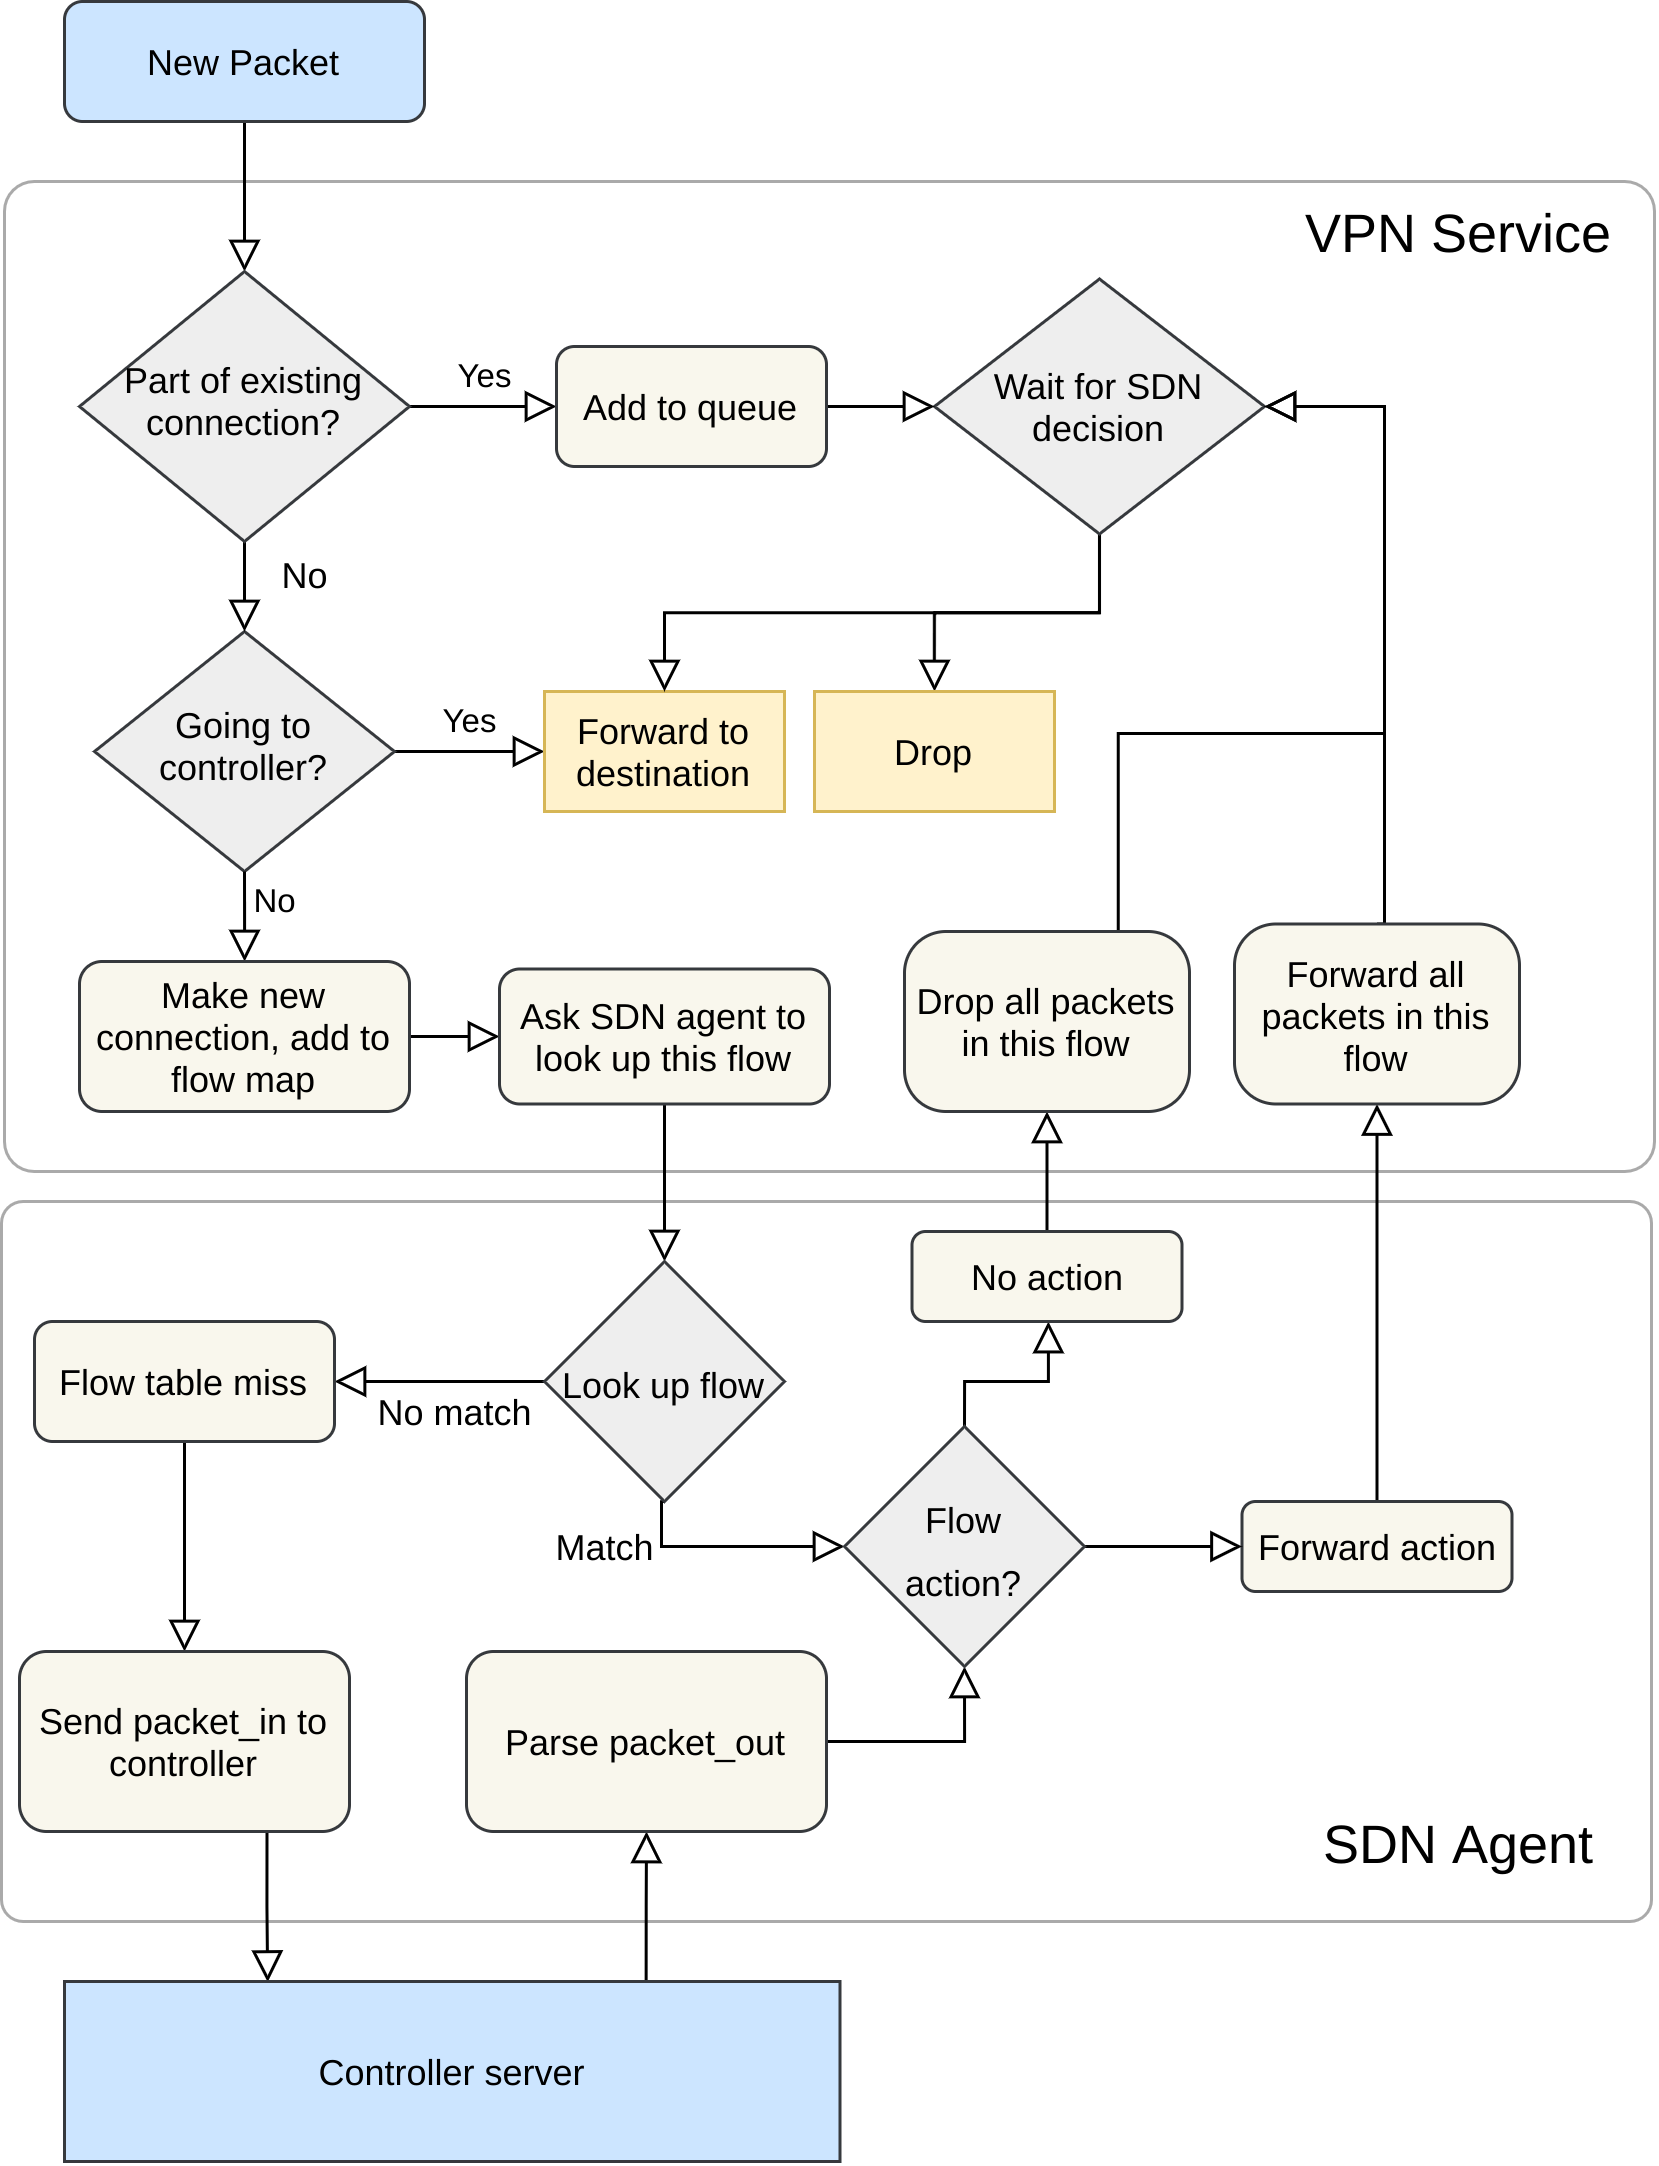
\includegraphics[width=0.9\textwidth]{sequence-diagram.png}
    \caption{Flow chart of the steps used to decide whether to forward or drop a
		packet.}
	\label{fig:packet-flow-chart}
\end{figure}


\subsection{Host-Based SDN}
\label{sec:host-based-sdn}

\textsc{Appjudicator} is designed to integrate with corporate SDN
infrastructure, so it needs to be able to communicate with an SDN controller
server. The OpenFlow switch specification, the de facto standard for
software-defined networking, describes a protocol for switch-controller
communication~\cite{openflowspec}. This specification is designed for large
network switches connected to potentially dozens of hosts, so implementing it on
a smartphone in Kotlin requires some special considerations.\footnote{Sections
\ref{sec:software-defined-networking} and 
\ref{sec:the-android-phone-as-an-sdn-agent} describe prior work in host-based
SDN agents on Android and other platforms.}

Large portions of the OpenFlow switch specification simply do not apply to
\textsc{Appjudicator}. For example, the app has no concept of Ethernet frames
and only one ``physical port'' in the sense that it is a switch for only one
host. \textsc{Appjudicator} does not support any optional features of the
specification. It can initiate a connection with an OpenFlow controller, report
its supported features, process \texttt{flow\_mod} messages, send
\texttt{packet\_in} messages, and receive \texttt{packet\_out} messages. We
provide more information on the OpenFlow specification in
Section~\ref{sec:openflow-protocol}.

\subsubsection{SDN Rule Cache}
\label{sec:implementation-sdn-rule-cache}

Like any SDN agent, \textsc{Appjudicator} maintains a cache of rules to apply to
network flows that pass through it. Rules can match any combination of source or
destination IP addresses, source or destination ports, and protocol, or have
wildcards for any of those fields. Each rule contains instructions on what types
of flows to match and a list of actions to perform on matched flows. We only
support the minimum allowed set of possible flow actions: forward and drop.

When a new connection is created, the VPN service notifies the SDN agent and
queues all packets from that flow until it gets a response from the SDN agent.
The SDN agent looks up the flow in its flow table. It finds the most specific
matching rule (\textit{i.e.}, the matching rule that had to use the fewest
wildcards) and sends its actions back to the VPN service. If no matching rule is
found in the flow table, the agent elevates the flow to the controller along
with UI context in a \texttt{packet\_in} message.
Figure~\ref{fig:packet-flow-chart} illustrates this process.
Section~\ref{sec:openflow-protocol} provides more information about
\texttt{packet\_in} and \texttt{packet\_out} messages.

\textsc{Appjudicator} will continue forwarding, blocking, or elevating packets
in other flows while waiting for a response from the SDN controller. The
controller makes a decision based on the network and UI context and sends back a
\texttt{packet\_out} response describing what to do with the flow.

\subsubsection{OpenFlow Protocol}
\label{sec:openflow-protocol}

The OpenFlow Switch Specification describes a protocol for SDN agents to connect
to a controller and exchange messages~\cite{openflowspec}. \textsc{Appjudicator}
implements the minimum subset of the OpenFlow Protocol (OFP). All OpenFlow
messages are sent over TCP in OpenFlow packets. These packets have a simple
8-byte header that describes the OpenFlow version, the type of the message, the
total length of the packet, and transaction ID (see
Figure~\ref{fig:openflow-header}). Replies to an OpenFlow message have the same
transaction ID as the request.

\begin{figure}[h]
    \centering
    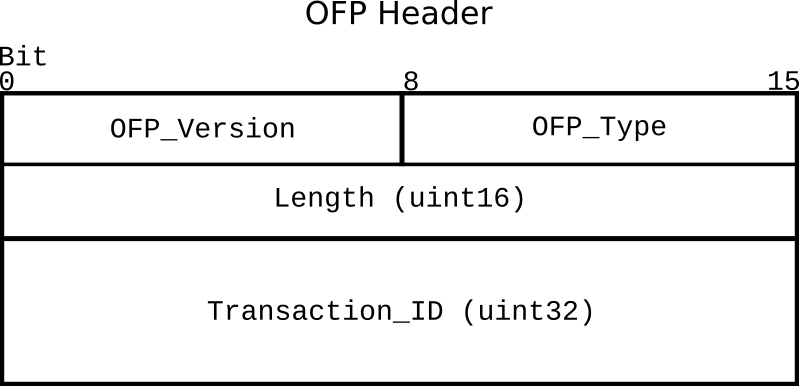
\includegraphics[width=.6\textwidth]{openflow-header.png}
    \caption{Fields of an OpenFlow packet header.}
    \label{fig:openflow-header}
\end{figure}

When the app is launched it opens a new TCP connection to a user-configurable IP
address or host name that runs the controller server. The controller and switch
each send a \texttt{hello} message to initiate the connection. The controller
then queries the switch to see what capabilities and features it supports.
\textsc{Appjudicator} replies with a \texttt{switch\_features} message
explaining that it has one physical port (the phone itself) and only supports
two packet actions: forward and drop. At this point the connection is fully
established, and the controller and agent can both send messages back and forth.
Figure~\ref{fig:openflow-handshake} depicts this process.

\begin{wrapfigure}{R}{0.4\textwidth}
	\centering
	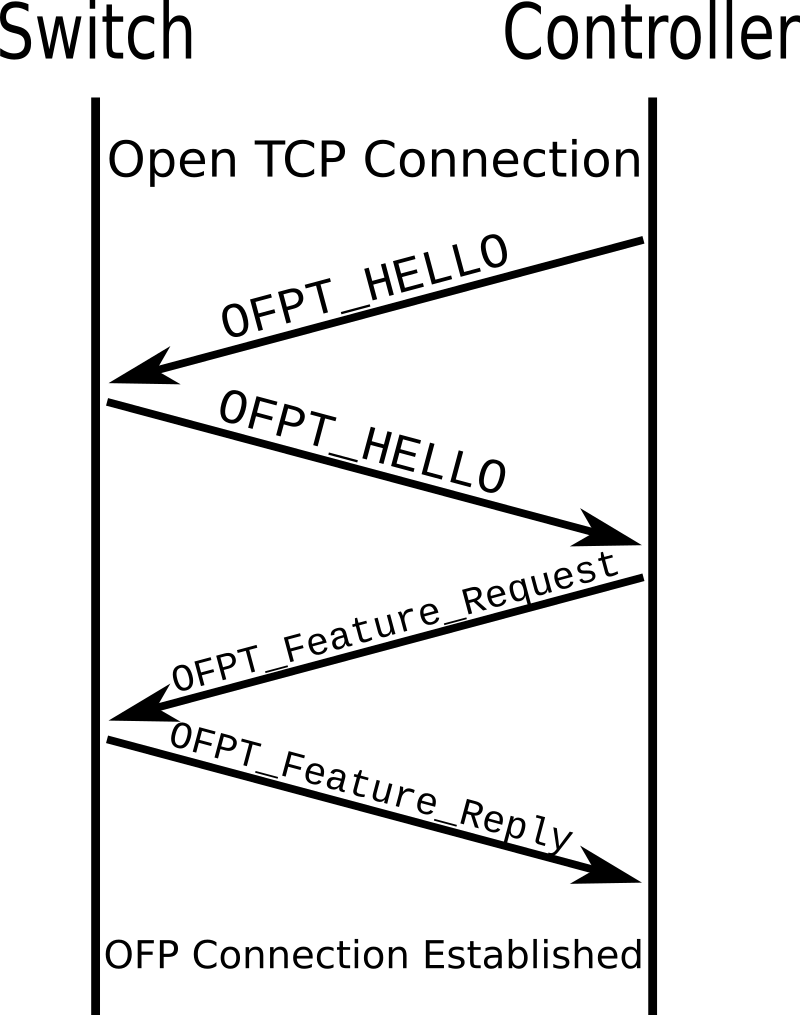
\includegraphics[width=0.4\textwidth]{openflow-handshake.png}
    \caption{OpenFlow handshake diagram.}
    \label{fig:openflow-handshake}
\end{wrapfigure}

While the app is running, the controller can modify flow rules on the
switch by sending a \texttt{flow\_mod} message. These instruct the switch
to add or remove one or more flow rules, and they are the primary way to enforce
new policy decisions.

The final type of communication between the SDN agent and controller is
\texttt{packet\_in}/\texttt{packet\_out} messages. When the SDN agent receives a
packet that does not match any flow rules, the agent must ask the controller
what to do with the packet. We construct a customized version of the standard
OFP \texttt{packet\_in} message to send to the controller, including UI
interaction metadata.\footnote{
	Section~\ref{sec:implementation-accessibility-service} describes how this
	metadata and how it is obtained.} Figure~\ref{fig:packet-in} shows the
fields included in these messages. The first eight bytes are the standard OFP
header. The ``buffer ID'' value will be included in the corresponding response
so the relevant packet can be identified.  The ``in port'' field do not apply to
host-based SDN agents like Appjudicator.  The reason field tells the controller
whether this \texttt{packet\_in} is being sent because of a flow table miss or
because an action explicitly requested sending the packet to the controller.

Appjudicator has no concept of link layer protocols, so the field for the
Ethernet header is zeroed out. Following this is the full contents of the IP
packet in question. Up to this point the \texttt{packet\_in} follows the
OpenFlow specification exactly, but after the packet contents we fill the rest
of the space available (up to 1500 bytes) with UI context, including UI events
from the same app that initiated the connection, their types, sources, and UI
hierarchy. IP packets sent to the controller will usually be the first packet of
a flow,\footnote{Such as a TCP SYN packet.} which are normally short, so
there may often be enough space to include the most relevant UI events.

The controller responds with a standard \texttt{packet\_out} message, which
tells the agent which actions to take on the flow. Optionally, the agent can
remember this response by adding a new flow table rule that matches the same
flow and applies the same actions so the controller will not have to be queried
again in the future. This is not part of the OpenFlow specification but is
feature of Appjudicator.

\subsubsection{Associating Network Flows with Context}
\label{sec:associating-network-flows-with-context}

When the SDN agent intercepts a new flow to a previously unknown domain, it
tries to associate it with UI context. The app looks up any accessibility events
from the past two seconds that originated from the same app that owns the
network connection (see Section~\ref{sec:deconstructing-flows}). We found that a
time interval of two seconds is long enough to catch most user-initiated network
requests without also associating unrelated UI interactions.

The app looks up any accessibility events that originated from the same package
that owns the connection that occurred in the two seconds before the flow was
initiated. If there is no likely initiator of the network flow (such as a button
press) within the two prior seconds, the flow is considered non-user-initiated.
The SDN agent includes information about these UI events, including the event
type and view hierarchy (see Section~\ref{sec:identifying-ui-elements}) with the
packet as it is elevated to the controller. This UI context should allow for
more powerful and fine-grained SDN rules.

\begin{figure}[h]
	\centering
	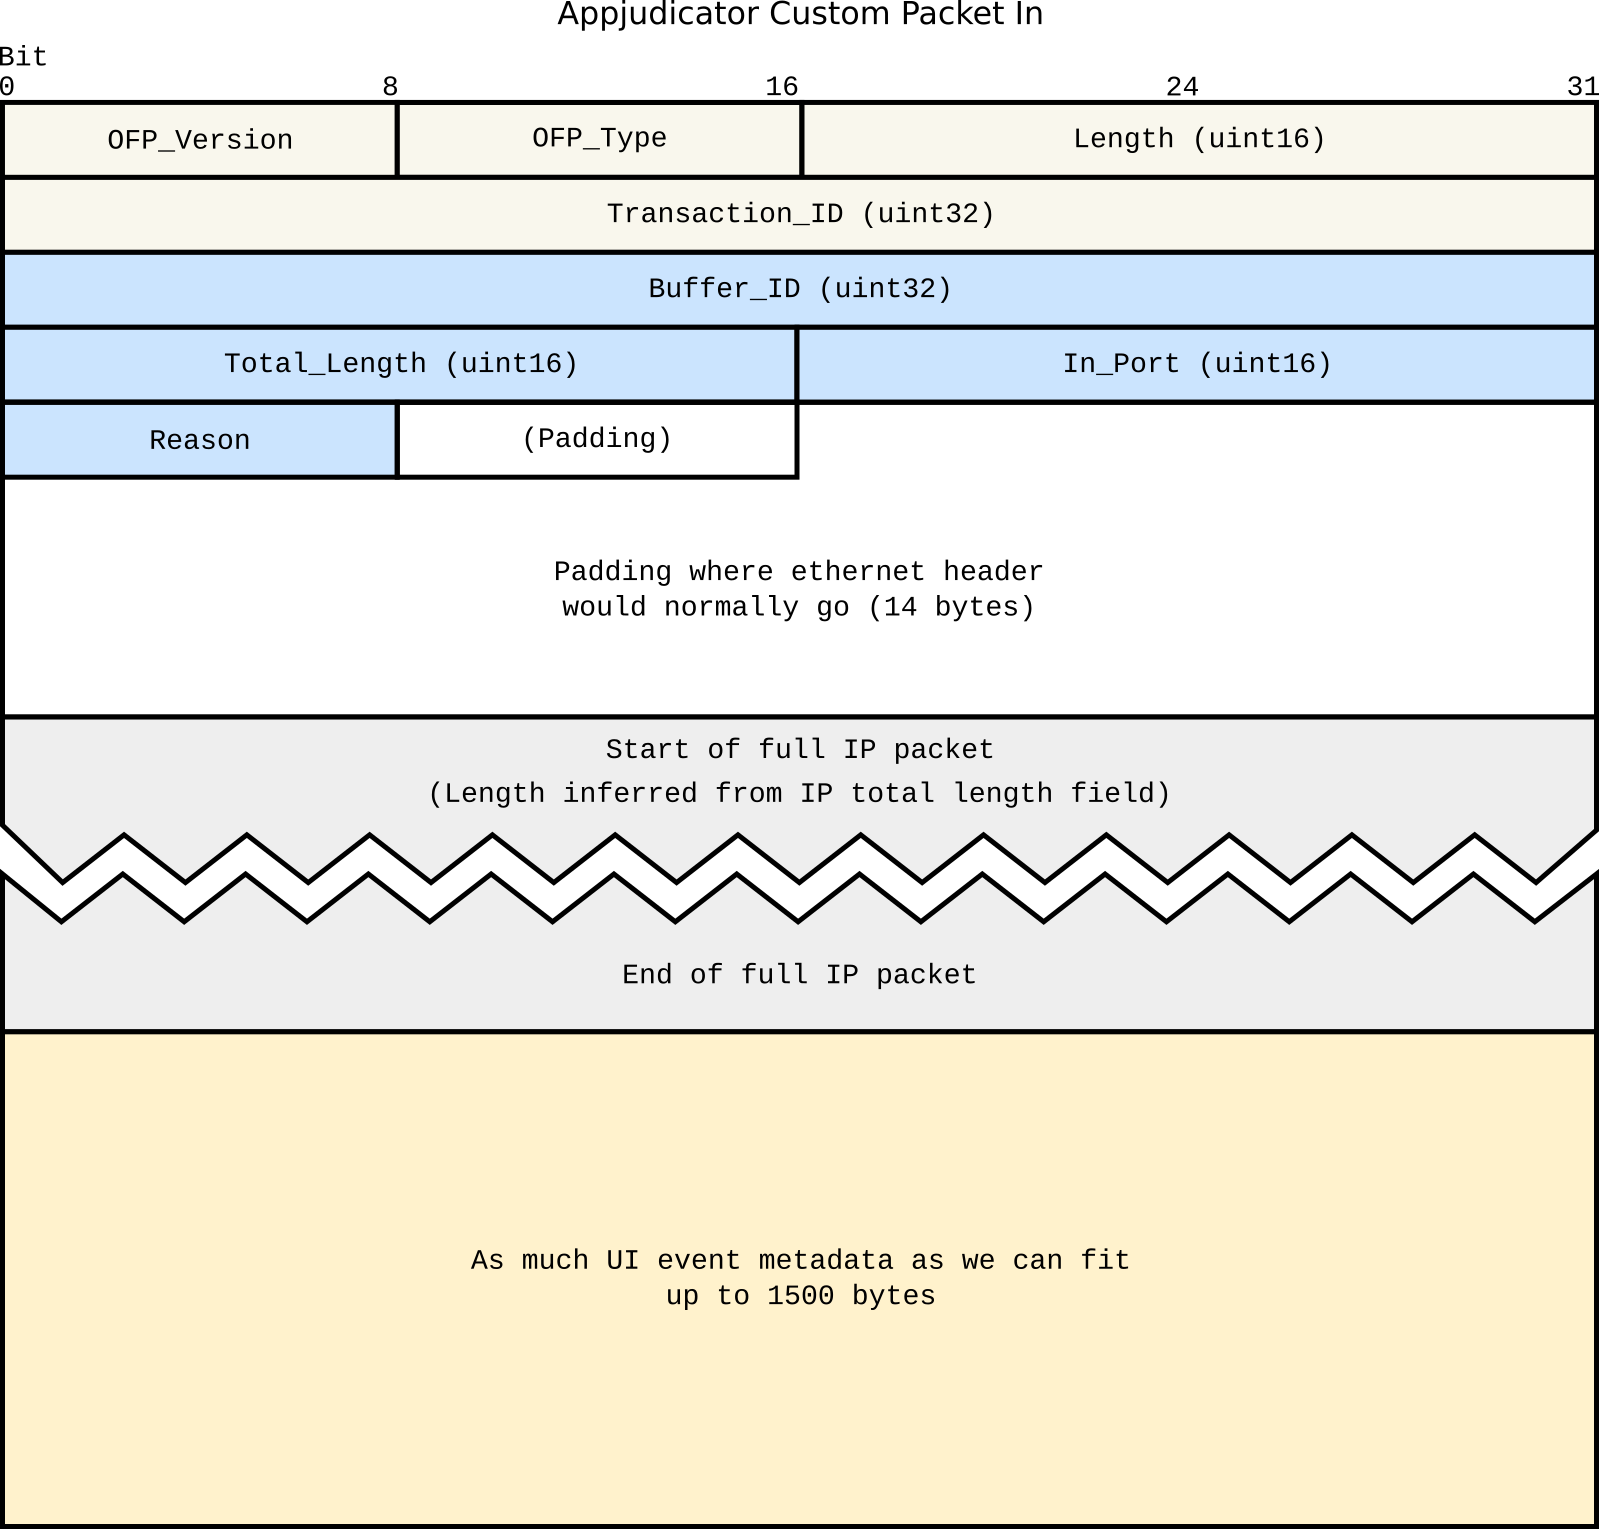
\includegraphics[width=0.9\textwidth]{packet-in.png}
    \caption{Fields in Appjudicator's custom \texttt{packet\_in} message.}
    \label{fig:packet-in}
\end{figure}

\subsubsection{Default-Allow Flows}
\label{sec:default-allow-flows}

Our system must account for non-user-initiated flows that occur as part of the
normal operation of the device. To do this, we profile the Android operating
system and common applications in advance.  While running in calibration mode,
\textsc{Appjudicator} adds the IP address and ports of all non-user-initiated
requests to a default-allow map. Then later, while operating normally, the app
will not question flows to these pairs of IP address and ports even if they are
not user-initiated.

% TODO what to do when controller is unavailable

\newpage

\section{Evaluation and Results}
\label{sec:evaluation-and-results}

We seek to evaluate whether \textsc{Appjudicator} is able to successfully
achieve its goal of distinguishing user-initiated network flows using UI
context, and whether it can do so with acceptable overhead. To determine whether
the app accomplishes its goal we perform a practical analysis and to measure the
app's resource cost we perform a performance evaluation. We now explain the
procedures used for each of these experiments and their results.

\subsection{Differentiating User-generated Flows}
\label{sec:differentiating-user-generated-flows}

The goal of this experiment is to determine whether \textsc{Appjudicator} can
successfully distinguish between network flows that were specifically initiated
by a human user and flows generated automatically by an app or the Android
system.

\subsubsection{Experimental Setup}
\label{sec:experimental-setup}

For this experiment, we tested the app both in an emulator an on a physical
Android device. The emulator test was performed on a virtual Google Pixel 4,
with API level 30 (the newest available). Physical tests were performed on a
real Google Pixel 3 phone running Android 11 with API level 30.

In both cases we used Google's UI Automator framework~\cite{uiautomator2020} to
automate the testing process. This tool is designed for automating UI tests as
part of an app development cycle, and provides features that make it ideal for
our experiments. The UI Automator can simulate various kinds of UI interactions,
including clicks, swipes, pressing hardware buttons, and even changing the
device's orientation. It can also perform actions in multiple apps in a single
run.

We use UI Automator to simulate a series of real life use cases that would lead
to a network request being made while \textsc{Appjudicator}'s accessibility
service is enabled. Then we simply check service's logs to see which flows it
marked as likely user-initiated. We run the test $x$ times to make sure the
results are reproducible, and not merely a coincidence of timing. See
Section~\ref{sec:practical-results} for the results of this experiment.

\subsubsection{Results}
\label{sec:practical-results}

% Use UI Automator to simulate real clicks, also find other apps that make background requests automatically
% Log whether each flow was user-generated, default-allowed, or automated
% What percentage of those flows were classified successfully?

\subsection{Performance Evaluation}
\label{sec:performance-evaluation}

To fulfill its purpose as an always-enabled enterprise network security tool,
\textsc{Appjudicator} has to be as unobtrusive to end users as possible. This is
especially important because the app performs some actions on every network
flow, so any latency added by it would be especially noticeable.

\subsubsection{Measuring Added Latency}
\label{sec:measuring-added-latency}

To measure the effect of \textsc{Appjudicator} on network communication speed,
we measure the total additional latency added by the app when initiating a TCP
connection.

For this test, we run the app in an Android virtual machine simulating a Google
Pixel 4, on API level 30. We use POX's \texttt{forwarding.hub} module as an
OpenFlow controller. In this mode, the controller responds to every query with
an instruction to forward the flow to its destination~\cite{mccauley2015}. Local
network latency is not a part of this test, so the controller server runs on the
same physical host as the Android virtual machine. The two components still
communicate over a regular TCP connection. The SDN agent starts with an empty
table of flow rules, so it must send a \texttt{packet\_in} to the controller for
every new flow. See Section~\ref{sec:openflow-protocol} for more information
about the OpenFlow protocol.

We measure the added latency of the first packet in a TCP connection because
this is where the system does the most processing. The start of a new flow
requires an SDN agent flow table lookup and possibly communication with the SDN
controller, and the app has to do more processing for TCP connections than UDP
connections. Subsequent packets in a TCP flow, and all packets in UDP flows
have lower latency.

We configure the app to log a timestamp when an outgoing TCP SYN packet is
intercepted from the device. \textsc{Appjudicator}'s VPN service then queues the
packet and asks the SDN agent what to do with it. The SDN agent tries to look up
the flow in its flow table and, finding no matching entry, sends a
\texttt{packet\_in} message to the controller. After the POX controller responds
with a \texttt{packet\_out} the SDN agent tells the VPN service to forward the
queued packets in the flow. Just before the initial SYN packet is sent to the
network a second timestamp is recorded. The earlier timestamp is the time the
packet would have been sent to the network without \textsc{Appjudicator}'s
influence, so the difference of these two timestamps is the total latency added
by the app.

There were 562 measured TCP connections during the sampling period and seven
removed as outliers, leaving 555 data points. The average added latency was 138
milliseconds, with a standard deviation of 38 milliseconds. In our sample 97\%
of TCP connections started with less than 200 milliseconds of added latency.
Figure~\ref{fig:tcp-delay-chart} charts the full results.

\begin{figure}[h]
    \centering
    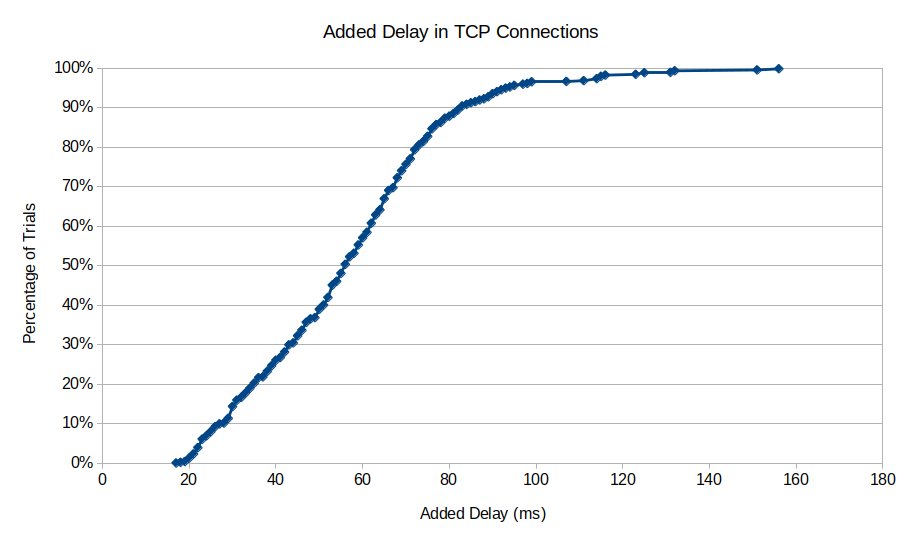
\includegraphics[width=\textwidth]{tcp-delay.png}
    \caption{Total latency added when initiating new TCP connections.}
	\label{fig:tcp-delay-chart}
\end{figure}

\subsubsection{Measuring Resource Overhead}
\label{sec:measuring-resource-overhead}


\newpage

\section{Conclusion}
\label{sec:conclusion}

\lipsum

\newpage


\label{sec:references}
%\printbibliography
\bibliographystyle{IEEEtranS}
\bibliography{references}

\end{document}
